\chapter{Planificación}

\vspace{-3mm}

A lo largo de este capítulo se describirán tanto el presupuesto requerido para el desarrollo del proyecto en base a los recursos hardware, software y humanos utilizados y se mostrará la temporización de las tareas en las que se ha fraccionado para su consecución.

% ********************************************************************

\section{Temporización}

El desarrollo del proyecto se ha estructurado en distintas fases de modo que se llevase a cabo un proceso iterativo. A continuación se ilustra el listado de tareas, así como su conexión con los objetivos establecidos anteriormente (\ref{item:objetivos}).

\vspace{-1mm}

\begin{itemize}
    \item \textbf{T1} - Elección del tema a desarrollar y línea de aprendizaje (10h)
    \item \textbf{T2} - Formación inicial (\ref{formacion}):
    \begin{itemize}
        \item \textbf{T2.1} - Curso Redes Neuronales y Aprendizaje profundo Coursera (30h)
        \item \textbf{T2.2} -  Curso \gls{NLP} Hugging Face (30h)
        \item \textbf{T2.3} -  Realización de \textit{walkthrougs} y máquinas \gls{CTF} (120h)
    \end{itemize}
    \item \textbf{T3} - Investigación sobre \textit{logs}, MITRE \gls{ATT&CK} y \gls{SIEM}s (30h) - \textbf{OBJ1.}
    \item \textbf{T4} - Implementación (I): Simulación de ataques y creación de \textit{dataset}- \textbf{OBJ2.}
    \begin{itemize}
        \item \textbf{T4.1} - Configuración del entorno (10h)
        \item \textbf{T4.2} - Elección de herramientas de simulación (5h)
        \item \textbf{T4.3} - Simulación de Ataques y Generación del Dataset (10h)
    \end{itemize}
    \item \textbf{T5} - Implementación (II): Preprocesado de \textit{datasets} (15h) - \textbf{OBJ2.} 
    \begin{itemize}
        \item \textbf{T5.1} - \textit{Dataset} propio
        \item \textbf{T5.2} - \textit{Dataset} Linux\_2k
        \item \textbf{T5.3} - \textit{Dataset} \gls{HDFS}
        \item \textbf{T5.4} - \textit{Dataset} \gls{BGL}
        \item \textbf{T5.5} - \textit{Dataset} sintético
    \end{itemize}
    \item \textbf{T6} - Implementación (III): Desarrollo del \textit{clustering} (25h) - \textbf{OBJ3.}
    \begin{itemize}
        \item \textbf{T6.1} - K-means
        \item \textbf{T6.2} - \gls{DBSCAN}
        \item \textbf{T6.3} - Hierarquical Clustering
    \end{itemize}
    \item \textbf{T7} - Análisis de Resultados obtenidos (5h)  - \textbf{OBJ4.}
    \begin{itemize}
        \item \textbf{T7.1} - Silhouette score
        \item \textbf{T7.2} - Índice de Davies-Bouldin
        \item \textbf{T7.3} - Índice de Cainski-Harabasz
    \end{itemize}
    \item \textbf{T8} - Redacción de la memoria (95h)  - \textbf{OBJ5.}
\end{itemize}

En función de las tareas indicadas, el tiempo estimado de esfuerzo para completar el proyecto es de \textbf{385h} aproximadamente. \\

\vspace{-4mm}

\subsubsection*{Diagrama de Gantt}

Para cumplimentar todas y cada una de las tareas, se ha desarrollado el Diagrama de Gantt ilustrado en la Figura \ref{fig:diagrama-gantt} entre los meses de septiembre de 2023 y junio de 2024, de modo que se alineen los esfuerzos en base al tiempo disponible y las tareas se fueran realizando periódicamente. Para ello, se han seguido las pautas indicadas por Raj Jain en el capítulo 5 de su libro \cite{jain1991art}. El diagrama ha sido realizado a través de Google Sheets por cuestiones de personalización, aunque existen herramientas automatizadas como GanttPRO \cite{GanttPRO} que facilitan su realización.

En dicho diagrama se pueden observar las distintas reuniones llevadas a cabo con los tutores para llevar un seguimiento de los pasos realizados y planificar las siguientes tareas a realizar, así como proponer mejoras y cambios en la implementación. 

Se ha hecho una división por bloques semanales, de modo que cada columna representa aproximadamente una semana del curso académico. En base al resultado obtenido, puede concluirse que el proyecto se ha realizado paulatinamente, aunque se puede observar un incremento considerable de la carga de trabajo durante los últimos dos meses.

\newpage

\begin{landscape}   
    \noindent\hspace*{-3.1cm}
    \begin{minipage}{\linewidth}
        \begin{figure}[H]
            \centering
            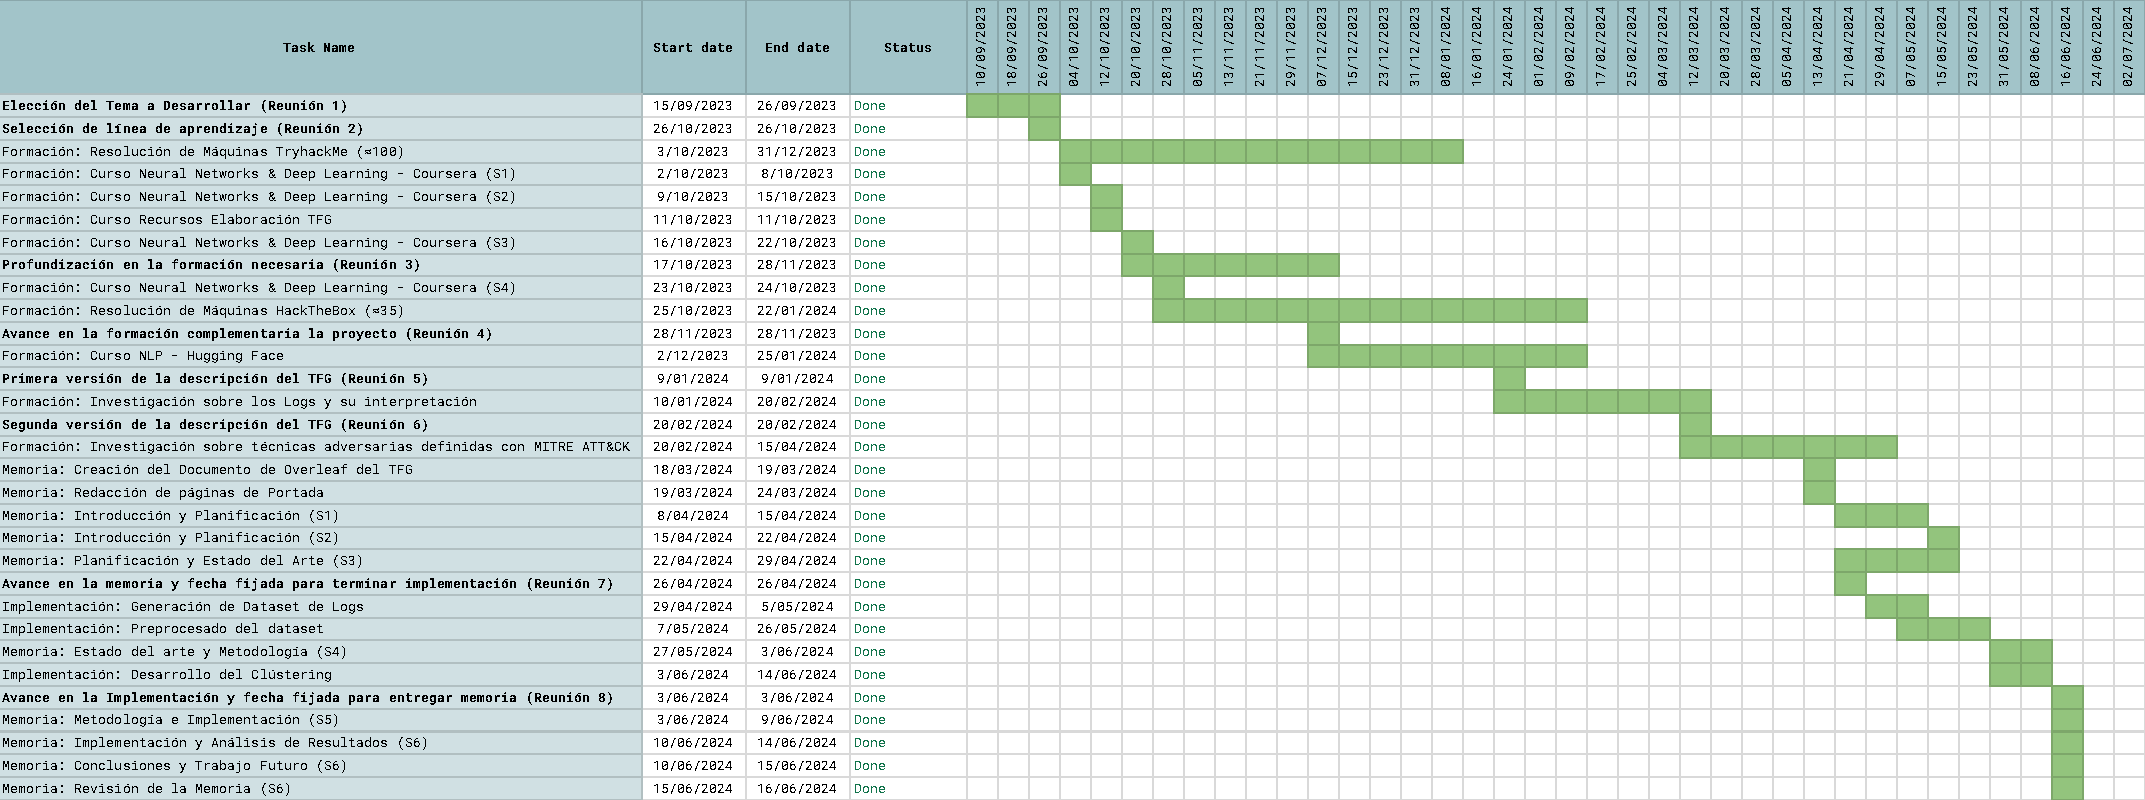
\includegraphics[width=1.3\linewidth, keepaspectratio]{imagenes/Diagrama de Gantt.png}
            \caption{Diagrama de Gantt}
            \label{fig:diagrama-gantt}
        \end{figure}
    \end{minipage}
\end{landscape}

\newpage

% ********************************************************************

\section{Presupuesto}

Para poder llevar a cabo el proyecto ha sido necesario realizar la planificación de los recursos a utilizar. En primer lugar establecer los recursos hardware, es decir, los dispositivos utilizados para el desarrollo de la memoria y de la implementación, así como los servicios de luz e internet. En segundo lugar, definir los recursos software: servicios en la nube, herramientas software, acceso a libros y artículos, etc. Finalmente, detallar el coste orientativo en recursos humanos en base al salario medio actual para un investigador en las áreas de Ciberseguridad e Inteligencia Artificial en función del tiempo invertido.

\begin{table}[H]
    \centering
    \footnotesize
    \begin{tabularx}{\linewidth}{|>{\raggedright\arraybackslash}X|r|}
    \hline
    \rowcolor{graylight}\texttt{Tipo de Recurso} & \texttt{Coste Total} \\
    \hline
    Recursos Hardware & 4.454,50\,\text{\euro} \\
    \hline
    Amortización Hardware & 411,75\,\text{\euro} \\
    \hline
    Recursos Software & 0\,\text{\euro} \\
    \hline
    Recursos Humanos & 19.545,80\,\text{\euro} \\
    \hline
    \textbf{Coste total} & \textbf{24.412,05\,\text{\euro}} \\ % Updated total cost
    \hline
    \end{tabularx}
    \caption{Presupuesto total del proyecto}
    \label{tab:presupuesto_total}
\end{table}


A continuación se desglosan cada uno de los elementos de la tabla indicando cómo se han realizado los cálculos.

\subsubsection*{Recursos Hardware}

En la siguiente tabla se detallan los recursos hardware utilizados, entre los que se incluyen un ordenador portátil y un ordenador de sobremesa, además del coste mensual para los servicios de luz e internet.

\begin{table}[H]
    \centering
    \footnotesize
    \begin{tabularx}{\linewidth}{|>{\raggedright\arraybackslash}X|c|c|c|}
    \hline
    \rowcolor{graylight}\texttt{Descripción} & \texttt{Uds.} & \texttt{Importe por unidad} & \texttt{Total} \\
    \hline
    Ordenador Portátil MSI Prestige 15 i7-1185G7 32GB RAM 1TB \gls{SSD} \gls{GTX} 1650 & 1 & 1.561,95 \euro & 1.561,95 \euro \\
    \hline
    Ordenador Sobremesa Intel i7-6700K 4.0Ghz 16GB RAM 1TB \gls{SSD} 1TB \gls{NVMe} \gls{GTX} 1080Ti 11GB \gls{GDDR}5X & 1 & 2.390,60 \euro & 2.390,60€ \\
    \hline
    Servicio de Internet (mensual) & 5 & 63,55 \euro& 317,75 \euro\\
    \hline
    Servicio de Luz (mensual) & 5 & 36,84 \euro & 184,20€ \\
    \hline
    \multicolumn{3}{|r|}{\textbf{Coste total}} & \textbf{4.454,50} \euro \\
    \hline
    \end{tabularx}
    \caption{Presupuesto hardware del Proyecto}
    \label{tab:presupuesto}
\end{table}

En base a un escenario realista, es necesario tener en cuenta la existencia de los costes de amortización. Según la normativa vigente, el porcentaje límite para la amortización de equipos de "Tratamiento de la Información y Sistemas y Programas Informáticos" se distribuye en un período de cuatro años \cite{fernandez2023amortizacion}. Considerando que el proyecto se ha desarrollado en un plazo aproximado de 5 meses, los costes de amortización serían de aproximadamente 411,75 \euro. \\

Para ello se han llevado a cabo los siguientes cálculos:

\begin{enumerate}
    \item Determinar el costo total de los equipos a amortizar:
    \[
    \text{Costo total de los equipos} = \text{Costo PC portátil} + \text{Costo PC sobremesa}
    \]
    \[
    \text{Costo total de los equipos} = 1.561,95 + 2.390,60 = 3.952,55 \ \text{\euro}
    \]

    \item Calcular la amortización anual:
    \[
    \text{Amortización anual} = \frac{\text{Costo total de los equipos}}{\text{Período de amortización en años}}
    \]
    \[
    \text{Amortización anual} = \frac{3.952,55}{4} = 988,14 \ \text{\euro}
    \]

    \item Calcular la amortización mensual:
    \[
    \text{Amortización mensual} = \frac{\text{Amortización anual}}{12}
    \]
    \[
    \text{Amortización mensual} = \frac{988,14}{12} = 82,35 \ \text{\euro}
    \]

    \item Calcular la amortización para 5 meses:
    \[
    \text{Amortización para 5 meses} = \text{Amortización mensual} \times 5
    \]
    \[
    \text{Amortización para 5 meses} = 82,35 \times 5 = 411,75 \ \text{\euro}
    \]
\end{enumerate}

\subsubsection*{Recursos Software}

En el caso de los recursos software, se ha utilizado únicamente servicios, herramientas y documentación de libre acceso. Por lo que el costo ha sido de 0€. Se ha hecho uso de los siguientes elementos:

\begin{table}[H]
    \centering
    \footnotesize
    \begin{tabularx}{\linewidth}{|l|X|}
    \hline
    \rowcolor{graylight}\texttt{Recurso} & \texttt{Detalles} \\
    \hline
    Recursos Bibliográficos & Accedidos a través de la cuenta institucional de la Universidad de Granada. Algunos ejemplos son Google Scholar, Science Direct y Scopus. \vspace{2mm}\\
    \hline
    Recursos de Internet & Accedidos a través de motores de búsqueda. Algunos ejemplos de los utilizados son Google, Firefox y DuckDuckGo. \vspace{2mm}\\
    \hline
    Conjuntos de datos & Accedidos a través de sitios web como GitHub, SecRepo y Kaggle. \vspace{2mm}\\
    \hline
    Herramientas de desarrollo & Plataformas de documentación como Overleaf e implementación como Google Colab \vspace{2mm}\\
    \hline
    \end{tabularx}
    \caption{Recursos software utilizados en el proyecto}
    \label{tab:recursos}
\end{table}

Los sistemas operativos utilizados para el desarrollo del proyecto son software libre, y están detallados en la primera sección del capítulo cinco (\ref{tab:machines}).

\subsubsection*{Recursos Humanos}

Para calcular el coste en recursos humanos, se ha considerado el salario medio de un investigador en Ciberseguridad e Inteligencia Artificial, que es de aproximadamente 30.000€ brutos anuales \cite{ufv2023cybersecurity}. El proyecto ha requerido un total de 385 horas de trabajo distribuidas en 5 meses.

\begin{enumerate}
    \item Determinar el salario mensual:
    \[
    \text{Salario mensual} = \frac{\text{Salario anual}}{12}
    \]
    \[
    \text{Salario mensual} = \frac{30.000\,€}{12} = 2.500 \ \text{\euro}
    \]

    \item Calcular el salario por hora (considerando una jornada laboral de 40 horas semanales):
    \[
    \text{Salario por hora} = \frac{\text{Salario mensual}}{160} \quad (\text{160 horas/mes})
    \]
    \[
    \text{Salario por hora} = \frac{2.500\,€}{160} = 15,63 \ \text{\euro}
    \]

    \item Calcular el coste total en recursos humanos, ajustando a un sobrecoste estimado entre un 200\% y 300\% para estudiantes:
    \[
    \text{Coste por hora (ajustado)} = \text{Salario por hora} \times 2.5
    \]
    \[
    \text{Coste por hora (ajustado)} = 15,63\,€ \times 2.5 = 39,08 \ \text{\euro} \quad (\text{Sobrecoste del 250\%})
    \]
    \[
    \text{Coste total en recursos humanos (estudiante)} = 39,08\,€ \times 385 = \textbf{15.045,80} \ \text{\euro}
    \]
\end{enumerate}

Es importante mencionar que el presupuesto asignado no es competitivo para la investigación que se quiere llevar a cabo. Generalmente, estas tareas son realizadas por expertos en la área, sin embargo este proyecto se formuló para ser ejecutado sin experiencia previa, con el principal objetivo de aprender durante el proceso. Como resultado, las tareas que un investigador experimentado podría completar en menos tiempo se extienden, lo que conlleva un aumento en los costos. \\

Además del gasto anterior, es necesario tener en cuenta el coste relativo a las horas de tutorización llevadas a cabo por los profesores asociadas a las reuniones llevadas a cabo y detalladas en el Diagrama de Gantt (\ref{fig:diagrama-gantt}), como aquellas destinadas a la corrección de esta memoria. Para realizar este cálculo deben contabilizarse las horas de esfuerzo y multiplicarse por el precio estimado por hora para un Profesor Titular de la Universidad de Granada \cite{ugr2023retribuciones}. Por tanto, este coste sería el siguiente:

\begin{enumerate}
\item Calcular el precio por hora para profesores, ajustando al sobrecoste que incluye los salarios en presupuestos:
\[
\text{Precio por hora} = 90 \text{ \euro} \quad (\text{Coste por hora típico en proyectos europeos})
\]

\item Calcular el coste total por cada profesor que tutoriza este trabajo:
\[
\text{Pablo García Sánchez} = 25 \text{ horas} \times 90 \text{ \euro / hora} = 2.250 \text{ \euro}
\]
\[
\text{Rafael Alejandro Rodríguez Gómez} = 25 \text{ horas} \times 90 \text{ \euro / hora} = 2.250 \text{ \euro}
\]
    \[
    \text{Total} = 4.500,00 \text{\euro}
    \]
\end{enumerate}

\textit{Fuente: Datos sobre retribuciones obtenidos de la Universidad de Granada} \cite{ugr2023retribuciones}.

\begin{table}[H]
    \centering
    \footnotesize
    \begin{tabularx}{\linewidth}{|>{\raggedright\arraybackslash}X|c|c|c|}
    \hline
    \rowcolor{graylight}\texttt{Descripción} & \texttt{Horas} & \texttt{Coste por hora} & \texttt{Coste Total} \\
    \hline
    Pablo García Sánchez (tutor) & 25 & 90 \text{\euro} & 2.250 \text{\euro} \\
    \hline
    Rafael Alejandro Rodríguez Gómez (cotutor) & 25 & 90 \text{\euro} & 2.250 \text{\euro} \\
    \hline
    \rowcolor{graylight}\multicolumn{3}{|r|}{\textbf{Coste total en tutorización}} & 4.500,00 \text{\euro} \\
    \hline
    \end{tabularx}
    \caption{Coste total de Recursos Humanos asociados a tutorización}
    \label{tab:coste-tutorizacion}
\end{table}

\footnotetext{Un trienio es un complemento de sueldo que se otorga por cada tres años de servicios prestados en la misma entidad, en reconocimiento a la experiencia y antigüedad acumulada.}




